\documentclass{sysuthesis}

%%
% 论文相关信息
% 本文档中前缀"c-"代表中文版字段, 前缀"e-"代表英文版字段
% modifyer: 黄俊杰(huangjj27, 349373001dc@gmail.com)
% update date: 2017-04-13
%%

% 标题
% 论文题目应以简短、明确的词语恰当概括整个论文的核心内容,避免使用不常见的缩略词、缩写字。读者通过标题可大致了解毕业设计(论文)的内容、专业的特点和科学的范畴。中文题目一般不宜超过 24 个字,必要时可增加副标题。外文题目一般不宜超过 12 个实词

% 封面标题。由于技术所限,封面题目过长的划分交由用户您进行定夺
% 这也能让您的论文封面看起来更有美感
\covertitlefirst{Lotka-Volterra模型在基因调控网络}
\covertitlesecond{与竞争型神经网络中的应用}

% Author:   Souler Ou
% 修改者:    欧一锋
% Date:     3/30/2018
% Mail:     ou@souler.cc
%如果英文标题过长可以使用此两项作为表三(答辩记录表)的标题。
\etitlefirst{Application of Lotka-Volterra Model in Gene Regulation Network}
\etitlesecond{and Competitive Neural Network}

% 另外一种封面的论文题目. 换行使用换行符("\\")
%\title{
%    中山大学 \\
%    本科毕业论文非正式模版
%}

% 中文标题
\ctitle{Lotka-Volterra模型在基因调控网络与竞争型神经网络中的应用}
\etitle{}

% 解决英文摘要页标题过长问题 (Issue 49&63)
% 当\etitle的长度超过页边距时,请使用下面的命令自行断行
% 此操作只影响英文摘要页的标题,不影响页眉的标题
% 如果不需要断行,将\eabstracttitlesecond{ }留空即可
\eabstracttitlefirst{Application of Lotka-Volterra Model in Gene Regulation Network} 
\eabstracttitlesecond{and Competitive Neural Network}

% 作者详细信息
\author{曾子奕}
\cauthor{曾\ 子\ 奕}    % 封面作者
\eauthor{Ziyi Zeng}
\studentid{14312056}
\cschool{工学院}

\cmajor{生物医学工程}
\emajor{Biomedical Engineering}

% 指导老师
\cmentor{唐承佩\ 教授}
\ementor{Prof. Tang}

     % 论文相关信息
%%
% 开题报告
% modifier: 黄俊杰(huangjj27, 349373001dc@gmail.com)
% update date: 2017-05-14

% 选题目的
\objective{

}

% 思路
\methodology{

}

% 研究方法/程序/步骤
\researchProcedure{

}

% 相关支持条件
\supportment{

}

% 进度安排
\schedule{

}

% 指导老师意见
\proposalInstructions{

}

   % 开题报告内容
%%
% 摘要信息
% 本文档中前缀"c-"代表中文版字段, 前缀"e-"代表英文版字段
% 摘要内容应概括地反映出本论文的主要内容,主要说明本论文的研究目的、内容、方法、成果和结论。要突出本论文的创造性成果或新见解,不要与引言相 混淆。语言力求精练、准确,以 300—500 字为宜。
% 在摘要的下方另起一行,注明本文的关键词(3—5 个)。关键词是供检索用的主题词条,应采用能覆盖论文主要内容的通用技术词条(参照相应的技术术语 标准)。按词条的外延层次排列(外延大的排在前面)。摘要与关键词应在同一页。
% modifier: 黄俊杰(huangjj27, 349373001dc@gmail.com)
% update date: 2017-04-15
%%

\cabstract{
摘要内容应概括地反映出本论文的主要内容,主要说明本论文的研究目的、内容、方法、成果和结论。要突出本论文的创造性成果或新见解,不要与引言相混淆。语言力求精练、准确,以300—500字为宜。在摘要的下方另起一行,注明本文的关键词(3—5个)。关键词是供检索用的主题词条,应采用能覆盖论文主要内容的通用技术词条(参照相应的技术术语标准)。按词条的外延层次排列(外延大的排在前面)。摘要与关键词应在同一页。
}
% 中文关键词(每个关键词之间用“;”分开,最后一个关键词不打标点符号。)
\ckeywords{本科毕业论文;\LaTeX\ 模板;中山大学}

\eabstract{
英文摘要内容与中文摘要相同,以250—400个实词为宜。摘要下方另起一行注明英文关键词(Keywords3—5个)。
}
% 英文文关键词(每个关键词之间用半角加空格分开, 最后一个关键词不打标点符号。)
\ekeywords{undergraduate thesis, \LaTeX\ template, Sun Yat-Sen University}

     % 摘要内容
%%
% 成绩评定记录表
% modifier: 黄俊杰(huangjj27, 349373001dc@gmail.com)
% update date: 2017-05-17

\gradingComment{
  某某同学针对什么问题研究了什么算法/实现了什么系统/针对这个系统做了什么测试,本文选题合理,实验结果表明技术路线……论文写作规范,引用文献充分,符合中山大学本科论文的规范,是篇优秀/良好/中等/合格的论文。
}
    % 成绩评定记录表评语
%%
% 四次进度报告相关信息

% Author:   Souler Ou
% 修改者:    欧一锋
% Date:     3/30/2018
% Mail:     ou@souler.cc

% 第一次进度报告
\firstsummary{
	\begin{adjustwidth}{2em}{2em}
		在这一阶段,XXX工作基本完成,主要在如下几个方面:
		\begin{enumerate}
			\item 完成了第一项。
			\item 完成了第二项
			\item 完成了第三项。 
		\end{enumerate}
	\end{adjustwidth}
}
% 第2次进度报告
\secondsummary{
	\begin{adjustwidth}{2em}{2em}
		...
	\end{adjustwidth}
}
% 第3次进度报告
\thirdsummary{
	\begin{adjustwidth}{2em}{2em}
		...
	\end{adjustwidth}
}
% 第4次进度报告
\fourthsummary{
	\begin{adjustwidth}{2em}{2em}
		...
	\end{adjustwidth}
}
% 第1次老师评价
\firstcomment{
	\begin{adjustwidth}{2em}{2em}
		论文完成情况良好。
	\end{adjustwidth}
}
% 第2次老师评价
\secondcomment{
	\begin{adjustwidth}{2em}{2em}
		...
	\end{adjustwidth}
}
% 第3次老师评价
\thirdcomment{
	\begin{adjustwidth}{2em}{2em}
		...
	\end{adjustwidth}
}
% 第4次老师评价
\fourthcomment{
	\begin{adjustwidth}{2em}{2em}
		...
	\end{adjustwidth}
}
% 老师总评价
\finalcomment{
	\begin{adjustwidth}{2em}{2em}
		...
	\end{adjustwidth}
}   % 过程检查报告数据
\begin{document}
    % 论文前置部分
    \frontmatter
        \pagenumbering{Roman}
        \maketitle    % 封面
        \makeProposal% 开题报告
        \makeProgressCheck  % 过程检查记录表
        \makeDefenseRecord  % 答辩情况等级表
        \makedisclaim       % 学术诚信声明
        \makeabstract       % 中英文摘要
        \maketableofcontents        % 目录
        \makelistoffiguretable

    % 论文主体部分
    \mainmatter
        % 引言

        % 正文
        %%
% 引言或背景
% 引言是论文正文的开端,应包括毕业论文选题的背景、目的和意义;对国内外研究现状和相关领域中已有的研究成果的简要评述;介绍本项研究工作研究设想、研究方法或实验设计、理论依据或实验基础;涉及范围和预期结果等。要求言简意赅,注意不要与摘要雷同或成为摘要的注解。
% modifier: 黄俊杰(huangjj27, 349373001dc@gmail.com)
% update date: 2017-04-15
%%

\chapter{引言}
%定义,过去的研究和现在的研究,意义,与图像分割的不同,going deeper
\label{cha:introduction}
\section{选题背景与意义}
\label{sec:background}
% What is the problem
% why is it interesting and important
% Why is it hards, why do naive approaches fails
% why hasn't it been solved before
% what are the key components of my approach and results, also include any specific limitations,do not repeat the abstract
%contribution
引言是论文正文的开端,应包括毕业论文选题的背景、目的和意义;对国内外研究现状和相关领域中已有的研究成果的简要评述;介绍本项研究工作研究设想、研究方法或实验设计、理论依据或实验基础;涉及范围和预期结果等。要求言简意赅,注意不要与摘要雷同或成为摘要的注解。

现代应用数学在向着“纯粹”和”应用“两大方向发展。即在最为抽象的领域中不断取得到优美定理的同时,又不断提供给应用科学和工程领域以解决问题的强有力的现代工具。将最新的抽象模型与计算成果应用于实际问题而得到具有指导意义的结果,是现代应用数学的一大特征。十分明显的,应用数学已经在生命科学,工程学以及计算机科学方面发挥着越来越重要的作用,抽象代数的引入为这些交叉学科问题不断提供着创新的解法和令人耳目一新的模型。

其中,Lotka-Volterra方程便是一个极为经典的例子。Lotka-Volterra方程的本质是n维空间上的微分方程与动力学建模。基于Lotka-Volterra方程的推导,定理,模型甚至一些猜想从第一次世界大战后直到今天一直都在蓬勃发展。

Lotka-Volterra方程其实并不是Lotka和Volterra合作提出的。而是最初由Alfred J. Lotka在1925年提出的,最初是描述植物物种和食草动物物种的种群关系。同样的方程组在1926年由数学物理学家Vito Volterra发表。Volterra的成果很大一部分是与海洋生物学家Umberto D'Ancona的共同实验得出的。D'Ancona研究了Adriatic海区的渔获量,并注意到在第一次世界大战期间捕获的掠食性鱼的比例有所增加(1914-1918)。这使他感到困惑,因为在战争期间,捕鱼的工作已经大大减少了。Volterra独立于Lotka开发了种群模型。有趣的是D'Ancona当时正在追求Volterra的女儿,公式发表之后D'Ancona迎娶了Volterra的女儿。

在1998年国际数学家大会召开时,Lotka-Volterra模型又迎来了一个里程碑式的进展。奥地利数学家J.Hofbauer和Karl.Sigmund将Lotka-Volterra微分方程与动力系统理论结合,提出了平均Liapunov函数方法。K.Sigmund以此为主题,在国际数学家大会上做了一小时全会报告。此后在1998到2010年间,基于Liapunov函数的Lotka-Volterra模型在应用数学领域得到了极大的发展。应用数学家们致力于研究基于Lotka-Volterra模型的常微系统的整体稳定性与持续生存性等问题,以及n维模型解析解的分析和讨论。比如最近提出的实根分离算法应用于三种群竞争系统极限环的算法化构造,得到了三个极限环的存在性证明。

可以说,最近十年里,以Lotka-Volterra方程为核心的应用数学分支发展突飞猛进,在生态学,博弈学,经济学,乃至社会科学都有很多应用。这种交叉学科的应用也很好解释:利用动力学的手段建模是非常合理的,真实生活行为的每种形式都是经过反复实验而成型的;这种逐步的适应性和通过个体的学习甚至自然选择都可以通过微分方程与动力学模拟。用数学语言表达即是:用未知量表征系统内每个对象,通过在连续时间上建立相互关系方程组,理论上就可以计算出任何时间的全部对象的状态。

Lotka-Volterra方程组及其衍生数学模型描述了系统中竞争,合作等不同模式的相互关系。有趣的是,当方程组的维数n=3时,已经没有解析解,我们只能通过分析解的性态

\section{国内外研究现状和相关工作}
\label{sec:related_work}
对国内外研究现状和相关领域中已有的研究成果的简要评述;
\section{本文的论文结构与章节安排}

\label{sec:arrangement}
本文共分为五章,各章节内容安排如下:

第一章引言。

第二章动力学模型,稳定性分析与分岔理论。

第三章两种群的捕食方程,竞争方程,解的性态。

第四章n种群的捕食方程,竞争方程,解的性态。

第五章应用一:基因调控网络

第六章应用二:竞争型神经网络与医学图像处理

第七章是本文的最后一章,总结与展望。是对本文内容的整体性总结以及对未来工作的展望。


        \newclearpage
        \chapter{动力学模型,稳定性分析与分岔理论}
\section{动力学模型}
本章主要目的是解释动力学的各个方面(长期的行为,平衡点,吸引盆,规则和不规则的振荡等等)。简单的单种群动力学模型可以表现出包括分岔和混沌在内的非常复杂的性态。
\section{系统中的相互作用}
任何一个系统中都存在研究对象之间的相互作用。生态系统更是如此。在很多生态系统中,上千类不同物种以复杂的模式相互作用。从一次近似的角度来看,我们可以抽象出三种不同的基本类型:(a)竞争:两个物种利用相同的资源,一个物种数量越多,对另一个物种就越不利。(b)互惠:物种之间彼此相互受益。真菌和藻类之间的共生,海葵和寄居蟹就属于这一类。(c)宿主-寄生关系:这是一种非对称关系。寄生物从宿主获利但对宿主无利。

由于竞争模式

\section{指数增长的离散与连续模型}
当然这是一种无限制增长,也是最简单的种群增长模型。
设\begin{math}R\end{math}为一个离散世代的种群增长率,即是说
\begin{align}
	\begin{split}
		\label{eq:feedforward}
		{x}'=Rx
	\end{split}
\end{align}

\begin{math}x\end{math}为某一世代的密度,而\begin{math}{x}'\end{math}为下一世代密度。如果\begin{math}R\end{math}为常数,则\begin{math}t\end{math}世代后的密度为\begin{math}R^{t}x\end{math},当\begin{math}R>1\end{math}时,表示爆炸式增长至无穷大。

当种群世代是连续的而不是离散的时候,我们设\begin{math}x(t)\end{math}为\begin{math}t\end{math}时刻的种群数量,则:
\begin{align*}
	\begin{split}
		\label{eq:feedforward}
		\frac{x\left ( t+\Delta t \right )-x\left ( t \right )}{\Delta t}
	\end{split}
\end{align*}
为时间区间\begin{math}\left [ t,t+\Delta t \right ]\end{math}的平均增长率。
\begin{align}
	\begin{split}
	\label{eq:feedforward}
	\frac{dx(t)}{dt}=\lim_{\Delta t\to 0}\frac{x(t+\Delta t)-x(t)}{\Delta t}
	\end{split}
\end{align}

在应用数学中,我们将其表示为\begin{math}\dot{x}(t)\end{math},将\begin{math}\frac{\dot{x}}{x}={log\ x}'\end{math}视为种群(单位)增长率。其含义为个体对种群增长率的平均贡献。本文统一用这一种表达记号。

指数增长中,其变化率为常数,即:
\begin{align}
	\begin{split}
	\label{eq:feedforward}
	\dot{x}=rx
\end{split}
\end{align}
\begin{align}
	\begin{split}
	\label{eq:feedforward}
	x(t)=x(0)e^{rt}
\end{split}
\end{align}

至此,对于离散和连续模型,我们都得到了指数增长。


\section{连续模型的Logistic增长}
在资源有限的情况下,\begin{math}r>1\end{math}的增长率都意味着种群随时间世代增加;较大的种群意味着较少的资源,又隐含了较少的增长率。此时增长率\begin{math}r\end{math}为\begin{math}x\end{math}的单调递减线性函数。即为形式\begin{math}r(1-\frac{x}{k})\end{math},其中\begin{math}r,k\end{math}为正常数。这就给出了Logistic方程

	\begin{align}
		\begin{split}
		\label{eq:feedforward}
		\dot{x}=rx\left ( 1-\frac{x}{k} \right )
	\end{split}
	\end{align}

通过线性代数与常微分方程的知识我们可以求解出(2.5)的通解为:
\begin{align}
	\begin{split}
	\label{eq:feedforward}
	x(t)=\frac{Kx(0)e^{rt}}{K+x(0)(e^{rt}-1)}
	\end{split}
\end{align}

根据通解,我们可以看出解的性态是容易分析的:如果\begin{math}x=0\end{math}或\begin{math}x=K\end{math},则\dot{x}为0;在这两种情况下,密度不会发生变化。当\begin{math}0<x<K\end{math}时,密度增加; \begin{math}x>K\end{math}时,密度减少。

\section{离散模型的递归关系}
某些昆虫可以视为世代不重叠种群。我们用\begin{math}y\end{math}和\begin{math}y'\end{math}分别表示某一代及下一代的种群量。类似上文我们用\begin{math}\frac{y'-y}{y}\end{math}表示其内禀单位增长率。类比Logistic增长公式,设其实际增长率为y的线性递减函数,则有:
	\begin{align}
		\begin{split}
		\label{eq:feedforward}
		y'=Ry\left (1- \frac{y}{K} \right )
		\end{split}
	\end{align}

对于这个离散模型,\begin{math}y'\end{math}与\begin{math}y\end{math}均不能超过其种群容纳量K,否则方程无意义。我们可以求解出当\begin{math}R>4\end{math}而\begin{math}y \to \frac{K}{2} \end{math},则\begin{math}y'>K\end{math},模型失去意义。因此我们限制\begin{math}R\in \left ( 0,4 \right )\end{math}。

这个有明显的缺陷的方程是否值得继续在本文中讨论呢?答案是肯定的。而推动接下来的讨论不是其生物学意义,而是这个简单动力学方程的解的性态有助于解释之后要引入的数学概念。
	
利用换元法,令\begin{math}x=\frac{y}{K},x'=\frac{y'}{K},r=\frac{R}{K}\end{math},我们可以得到差分方程\begin{math}x'=F(x)\end{math},
	\begin{align*}
		\begin{split}
		\label{eq:feedforward}
		F(x)=Rx(1-x)
		\end{split}
	\end{align*}

	接下来一节,我们通过这个最简单的非线性递归关系解的性态讨论其复杂的动力学性态,并引入三个重要的概念:稳定点,分岔与混沌。

\section{稳定和不稳定不动点}
我们考虑\begin{math}R\end{math}在0到4之间,映射
	\begin{align}
		\begin{split}
		\label{eq:feedforward}
		x\rightarrow Rx(1-x)
	\end{split}
	\end{align}
在区间\begin{math}\left [ 0,1 \right ]\end{math}定义了一个动力系统。当\begin{math}R\leqslant 1\end{math},对所有\begin{math}
x\end{math}都有\begin{math}x'<x\end{math},\begin{math}x\end{math}的轨道单调减小趋于0.所以我们仅讨论\begin{math}x>1\end{math}。

此时\begin{math}F\end{math}为一抛物线与\begin{math}x\end{math}轴交于0和1,在\begin{math}\frac{1}{2}\end{math}处达到其最大值。显然0是一个不动点。\begin{math}F\end{math}与对角线\begin{math}y=x\end{math}定义域中交于唯一点\begin{math}P\end{math},横坐标\begin{math}p=\frac{R-1}{R}\end{math}.

我们可以计算看看P的性态:

由均值定理
\begin{align*}
	\begin{split}
	\label{eq:feedforward}
	F(x)-p=F(x)-F(p)=(x-p)\frac{\mathrm{d} F(c)}{\mathrm{d} x}
\end{split}
\end{align*}

即\begin{math}\exists c\in [x,p]\end{math}使上式成立。

如果\begin{math}\left | \frac{\mathrm{d} F(p)}{\mathrm{d} x} \right |<1\end{math},则\begin{math}\left | \frac{\mathrm{d} F(c)}{\mathrm{d} x} \right |<1\end{math},在\begin{math}x\rightarrow c\end{math}(从而c)的时候成立。即有

\begin{align*}
	\begin{split}
	\label{eq:feedforward}
	\left | F(x)-p \right |<\left | x-p \right |
\end{split}
\end{align*}
即\begin{math}x'\end{math}比\begin{math}x\end{math}更接近\begin{math}P\end{math},即\begin{math}x\end{math}在合适的邻域收敛于\begin{math}p\end{math}。我们称此时\begin{math}P\end{math}是渐近稳定的。

类似的,如果\begin{math}\left | \frac{\mathrm{d} F(p)}{\mathrm{d} x} \right |>1\end{math},则
	\begin{align*}
		\begin{split}
		\label{eq:feedforward}
		\left | F(x)-p \right |>\left | x-p \right |
	\end{split}
	\end{align*}

即\begin{math}x\end{math}的轨道离开不动点,此时\begin{math}P\end{math}不是稳定点。

求解方程\begin{math}F(x)=Rx(1-x)\end{math}得\begin{math}\frac{\mathrm{d} F(p)}{\mathrm{d} x}=2-R\end{math}.即当\begin{math}1<R<3\end{math},\begin{math}P\end{math}为渐近稳定;但当\begin{math}3<R<4\end{math}是为不稳定。


\section{分岔}
当问题变成两个世代的时候,即\begin{math}x\end{math}的映射为\begin{math}F(F(x))=F^{(2)}(x)\end{math}.此时\begin{math}F^{(2)}(x)\end{math}为四次多项式,其局部极小在\begin{math}\frac{1}{2}\end{math}处,两个局部极大值对称地在\begin{math}\frac{1}{2}\end{math}的左右。对角线\begin{math}y=x\end{math}与\begin{math}F^{(2)}(x)\end{math}仍然交于\begin{math}p\end{math}。此时\begin{math}p\end{math}处的导数为\begin{math}(2-R)^{2}\end{math}。我们称此时

如果\begin{math}1<R<3\end{math},即\begin{math}P\end{math}是渐近稳定的,则对角线与\begin{math}F^{(2)}(x)\end{math}唯一交点即为\begin{math}P\end{math};如果\begin{math}3<R<4\end{math},\begin{math}P\end{math}斜率大于1,则可以得到另外两个交点。这两个交点对应于周期2点\begin{math}p1,p2\end{math}。

接下来利用解的性态看一下周期的解的性态:

如果存在\begin{math}k>1\end{math}使得\begin{math}T^{k}x=x\end{math},整数\begin{math}k\end{math}称为\begin{math}x\end{math}的周期。

研究周期解与稳定点可以得到很多有趣的性质:在模型(2.8)中,增长的变化具有一个世代的滞后。这种“滞后”导致的行为过渡,比如从不动点的一端跳到另一端,产生振荡而不能稳定下来。
        \newclearpage
        \chapter{研究方法}
\label{cha:method}

        \newclearpage
        %% chapter 4 dataset, network structure, experiment and result
\chapter{实验与结果}
\label{cha:experiment}


        \newclearpage
        %%
% 结论
% 结论是毕业论文的总结,是整篇论文的归宿,应精炼、准确、完整。结论应着重阐述自己的创造性成果及其在本研究领域中的意义、作用,还可进一步提出需要讨论的问题和建议。
% modifyer: 黄俊杰(huangjj27, 349373001dc@gmail.com)
% update date: 2017-04-13
%%

\chapter{总结与展望}
\section{工作总结}
\section{研究展望}

        \newclearpage
        % 结语

    % 附录部分
    \backmatter
        % 参考文献. 因不需要纳入章节目录, 故放入附录部分
        % 实际上参考文献是属于论文主体部分
        \makereferences

        %%
% 致谢
% 谢辞应以简短的文字对课题研究与论文撰写过程中曾直接给予帮助的人员(例如指导教师、答疑教师及其他人员)表示对自己的谢意,这不仅是一种礼貌,也是对他人劳动的尊重,是治学者应当遵循的学术规范。内容限一页。
% modifier: 黄俊杰
% update date: 2017-04-15
%%

\chapter{致谢}

	四年时间转眼即逝,青涩而美好的本科生活快告一段落了。回首这段时间,我不仅学习到了很多知识和技能,而且提高了分析和解决问题的能力与养成了一定的科学素养。虽然走过了一些弯路,但更加坚定我后来选择学术研究的道路,实在是获益良多。这一切与老师的教诲和同学们的帮助是分不开的,在此对他们表达诚挚的谢意。

	首先要感谢的是我的指导老师林倞教授。我作为一名本科生,缺少学术研究经验,不能很好地弄清所研究问题的重点、难点和热点,也很难分析自己的工作所能够达到的层次。林老师对整个研究领域有很好的理解,以其渊博的知识和敏锐的洞察力给了我非常有帮助的方向性指导。他严谨的治学态度与辛勤的工作方式也是我学习的榜样,在此向林老师致以崇高的敬意和衷心的感谢。

	最后我要感谢我的家人,正是他们的无私的奉献和支持,我才有了不断拼搏的信息的勇气,才能取得现在的成果。

\vskip 108pt
\begin{flushright}
	陈冠英\makebox[1cm]{} \\
\today
\end{flushright}

    % 致谢
        \newclearpage
        % 附录
    \appendix
        \chapter{补充更多细节}

\begin{figure}[h!]
\centering
		\makebox[0.16\textwidth]{\scriptsize 图像}
		\makebox[0.16\textwidth]{\scriptsize 真值}
		\makebox[0.16\textwidth]{\scriptsize Grid-5LSTM1}
		\makebox[0.16\textwidth]{\scriptsize Grid-5LSTM3}
		\makebox[0.16\textwidth]{\scriptsize Grid-5LSTM5} \\
		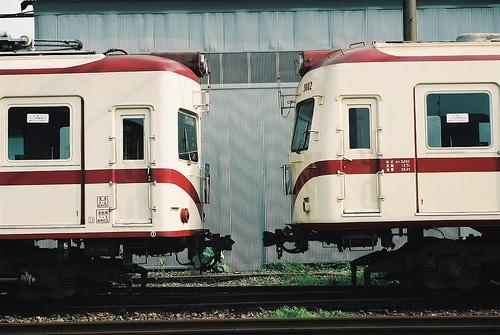
\includegraphics[width=0.16\textwidth]{image/appendix1/2007_000042.jpg}
		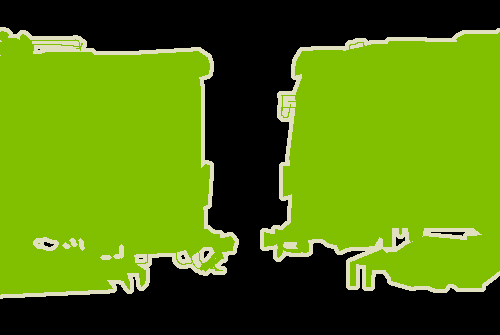
\includegraphics[width=0.16\textwidth]{image/appendix1/2007_000042.png}
		
\includegraphics[width=0.16\textwidth]{image/appendix1/1/2007_000042.png} 
		
\includegraphics[width=0.16\textwidth]{image/appendix1/3/2007_000042.png}
		
\includegraphics[width=0.16\textwidth]{image/appendix1/5/2007_000042.png} \\

		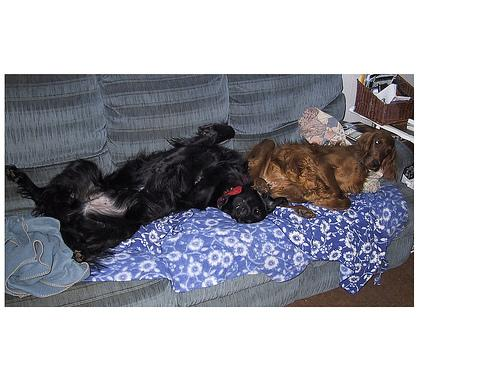
\includegraphics[width=0.16\textwidth]{image/appendix1/2011_003256.jpg}
		
\includegraphics[width=0.16\textwidth]{image/appendix1/2011_003256.png}
		
\includegraphics[width=0.16\textwidth]{image/appendix1/1/2011_003256.png} 
		
\includegraphics[width=0.16\textwidth]{image/appendix1/3/2011_003256.png}
		
\includegraphics[width=0.16\textwidth]{image/appendix1/5/2011_003256.png} \\
		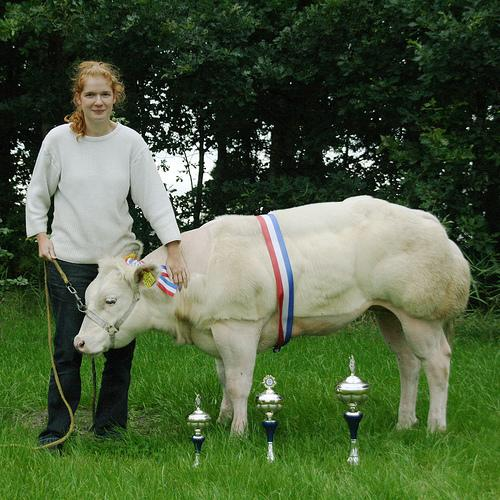
\includegraphics[width=0.16\textwidth]{image/appendix1/2011_001159.jpg}
		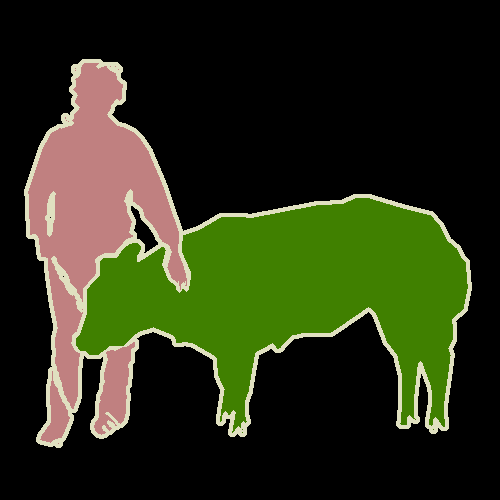
\includegraphics[width=0.16\textwidth]{image/appendix1/2011_001159.png}
		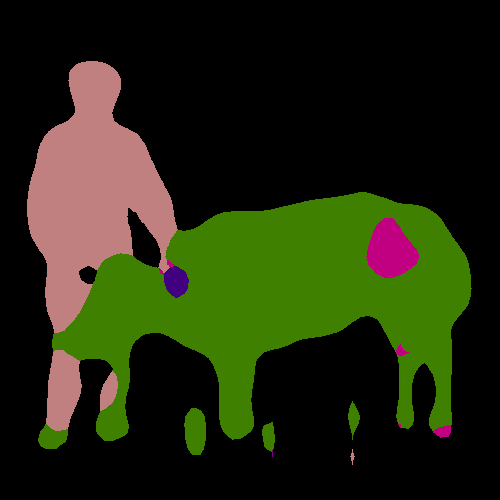
\includegraphics[width=0.16\textwidth]{image/appendix1/1/2011_001159.png} 
		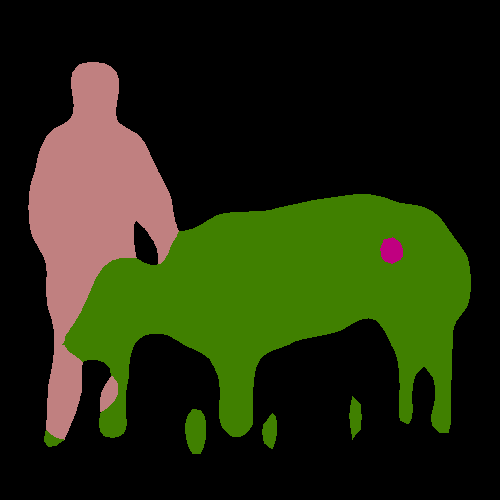
\includegraphics[width=0.16\textwidth]{image/appendix1/3/2011_001159.png}
		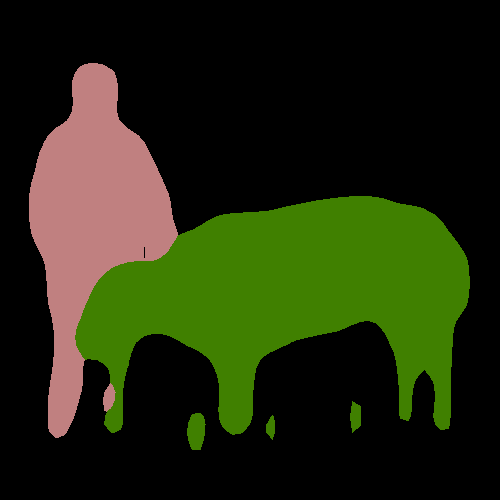
\includegraphics[width=0.16\textwidth]{image/appendix1/5/2011_001159.png} \\
		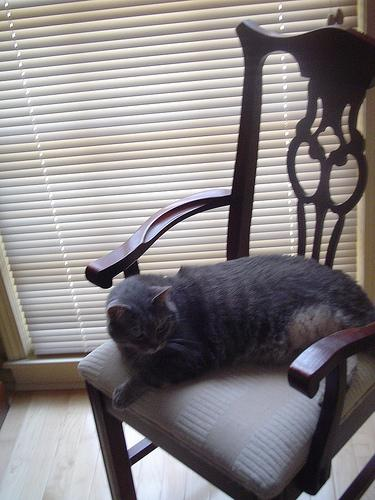
\includegraphics[width=0.16\textwidth]{image/appendix1/2011_000813.jpg}
		
\includegraphics[width=0.16\textwidth]{image/appendix1/2011_000813.png}
		
\includegraphics[width=0.16\textwidth]{image/appendix1/1/2011_000813.png} 
		
\includegraphics[width=0.16\textwidth]{image/appendix1/3/2011_000813.png}
		
\includegraphics[width=0.16\textwidth]{image/appendix1/5/2011_000813.png} \\
		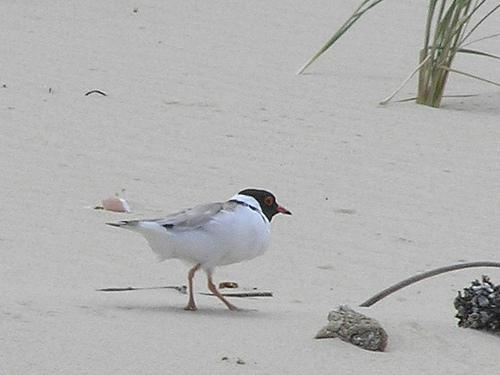
\includegraphics[width=0.16\textwidth]{image/appendix1/2011_003145.jpg}
		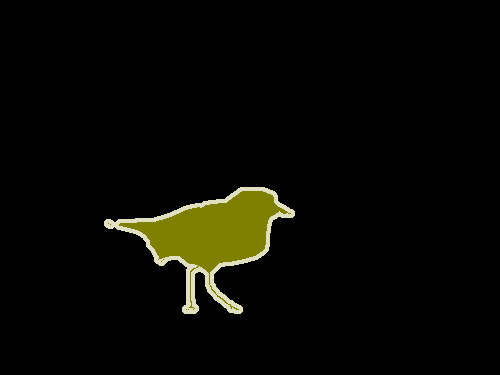
\includegraphics[width=0.16\textwidth]{image/appendix1/2011_003145.png}
		
\includegraphics[width=0.16\textwidth]{image/appendix1/1/2011_003145.png} 
		
\includegraphics[width=0.16\textwidth]{image/appendix1/3/2011_003145.png}
		
\includegraphics[width=0.16\textwidth]{image/appendix1/5/2011_003145.png} \\
		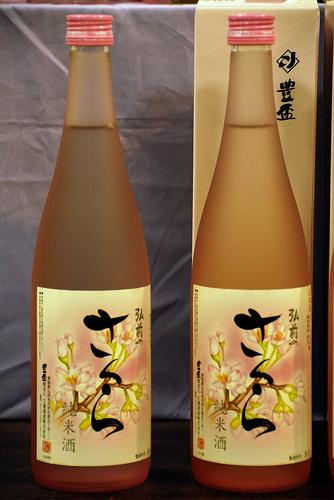
\includegraphics[width=0.16\textwidth]{image/appendix1/2009_004579.jpg}
		
\includegraphics[width=0.16\textwidth]{image/appendix1/2009_004579.png}
		
\includegraphics[width=0.16\textwidth]{image/appendix1/1/2009_004579.png} 
		
\includegraphics[width=0.16\textwidth]{image/appendix1/3/2009_004579.png}
		
\includegraphics[width=0.16\textwidth]{image/appendix1/5/2009_004579.png} \\
\color[rgb]{0.9,0.9,0.9}\bfseries
\begin{tabular}{*{7}{>{\centering\arraybackslash}p{0.10\textwidth}}}
	\hline
	\cellcolor[rgb]{0,0,0}  背景&\cellcolor[rgb]{0.5020,0,0} 飞机 &\cellcolor[rgb]{0,0.5020,0} 自行车 &\cellcolor[rgb]{0.5020,0.5020,0} 鸟 &\cellcolor[rgb]{0,0,0.5020} 船   &\cellcolor[rgb]{0.5020,0,0.5020} 瓶子 &\cellcolor[rgb]{0,0.5020,0.5020} 大巴
	\\
	\hline
	\cellcolor[rgb]{0.5020,0.5020,0.5020} 汽车 & \cellcolor[rgb]{0.2510,0,0} 猫 &\cellcolor[rgb]{0.7529,0,0} 椅子 &\cellcolor[rgb]{0.2510,0.5020,0} 牛 &\cellcolor[rgb]{0.7529,0.5020,0} 桌子 &\cellcolor[rgb]{0.2510,0,0.5020} 狗 &\cellcolor[rgb]{0.7529,0,0.5020} 马 \\
	\hline
	\cellcolor[rgb]{0.2510,0.5020,0.5020} 摩托车 &\cellcolor[rgb]{0.7529,0.5020,0.5020} 人   &\cellcolor[rgb]{0,0.2510,0} 盆栽   &\cellcolor[rgb]{0.5020,0.2510,0} 羊 &\cellcolor[rgb]{0,0.7529,0} 沙发 &\cellcolor[rgb]{0.5020,0.7529,0} 火车 &\cellcolor[rgb]{0,0.2510,0.5020} 电视 \\
	\hline
\end{tabular}

\caption{一个配有彩色表格的插图}
\end{figure}

\endinput

        \newclearpage
    \makeGrade      % 成绩评定记录表
\end{document}

